\newcommand{\entree}{effort résistant des bocaux $F_b$}
\newcommand{\delentree}{de l'\entree}
\newcommand{\lentree}{l'\entree}
\newcommand{\sortie}{couple moteur $C_m$}
\newcommand{\delasortie}{du \sortie}
\newcommand{\lasortie}{le \entree}
\newcommand{\correction}{
\begin{center}
 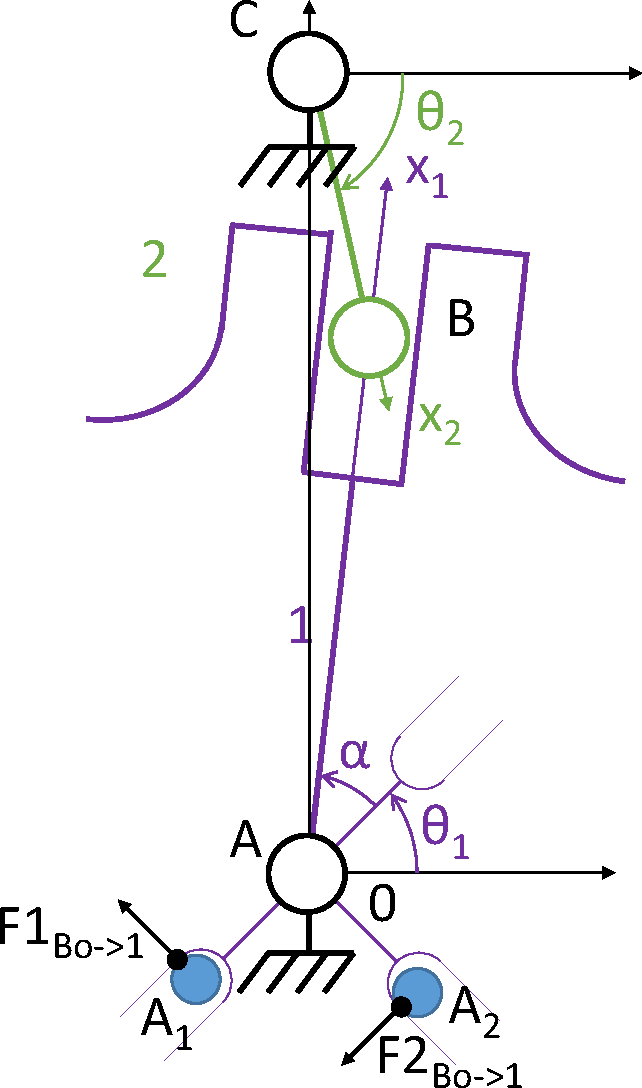
\includegraphics[width=0.4\linewidth]{img/Capsuleuse_cin}
\end{center}

$\left\{T_{Bo\rightarrow 1}\right\}=\left\{\begin{array}{cc}
-F_B & \sim \\
0 & \sim \\
\sim & 0
\end{array}\right\}_{A_2,R_1}+
\left\{\begin{array}{cc}
0 & \sim \\
F_B & \sim \\
\sim & 0
\end{array}\right\}_{A_1,R_1}$

$\left\{T_{Bo\rightarrow 1}\right\}=
\left\{\begin{array}{cc}
-F_B & \sim \\
F_B & \sim \\
\sim & -F_B.(2.R_c+l.(cos\alpha+sin\alpha))
\end{array}\right\}_{B,R_1}$

$\left\{T_{Bo\rightarrow 1}\right\}=
\left\{\begin{array}{cc}
-F_B.(cos\theta_1+sin\theta_1) & \sim \\
-F_B.(sin\theta_1-cos\theta_1) & \sim \\
\sim & -F_B.(2.R_c+l.(cos\alpha+sin\alpha))
\end{array}\right\}_{B,R}$

$\left\{T_{C_m\rightarrow 2}\right\}=
\left\{\begin{array}{cc}
0 & \sim \\
0 & \sim \\
\sim & C_m
\end{array}\right\}_B$

$\left\{T_{0\rightarrow 1}\right\}=\left\{\begin{array}{cc}
X_{01} & \sim \\
Y_{01} & \sim \\
\sim & 0
\end{array}\right\}_A=
\left\{\begin{array}{cc}
X_{01} & \sim \\
Y_{01} & \sim \\
\sim & -l.cos(\alpha+\theta_1).Y_{01}+l.sin(\alpha+\theta_1).X_{01}
\end{array}\right\}_B$

$\left\{T_{0\rightarrow 2}\right\}=\left\{\begin{array}{cc}
X_{02} & \sim \\
Y_{02} & \sim \\
\sim & 0
\end{array}\right\}_C=
\left\{\begin{array}{cc}
X_{02} & \sim \\
Y_{02} & \sim \\
\sim & -R.cos(\theta_2).Y_{02}+R.sin(\theta_2).X_{02}
\end{array}\right\}_B$

$\left\{T_{1\rightarrow 2}\right\}=\left\{\begin{array}{cc}
0 & \sim \\
Y_{12} & \sim \\
\sim & 0
\end{array}\right\}_{B,R_1^*}=
\left\{\begin{array}{cc}
-sin(\alpha+\theta_1).Y_{12} & \sim \\
cos(\alpha+\theta_1).Y_{12} & \sim \\
\sim & 0
\end{array}\right\}_{B,R_0}$

Isoler 1

$\left\{\begin{array}{l}
-F_B.(cos\theta_1+sin\theta_1)+X_{01}+sin(\alpha+\theta_1).Y_{12}=0 \\
-F_B.(sin\theta_1-cos\theta_1)+Y_{01}-cos(\alpha+\theta_1).Y_{12}=0 \\
-F_B.(2.R_c+l.(cos\alpha+sin\alpha))-l.cos(\alpha+\theta_1).Y_{01}+l.sin(\alpha+\theta_1).X_{01}=0
\end{array}\right.$

Isoler 2

$\left\{\begin{array}{l}
X_{02}-sin(\alpha+\theta_1).Y_{12}=0 \\
Y_{02}+cos(\alpha+\theta_1).Y_{12}=0 \\
C_m-R.cos\theta_2.Y_{02}+R.sin\theta_2.X_{02}=0
\end{array}\right.$

Donc, $Y_{12}=-\frac{F_B.2.R_c}{l}$

Donc $C_m=R.\frac{F_B.2.R_c}{l}.cos(\theta_1-\theta_2+\alpha)$
}

